\documentclass[border=10pt]{standalone}
\usepackage{tikz}
\usetikzlibrary{arrows.meta,positioning}

\begin{document}

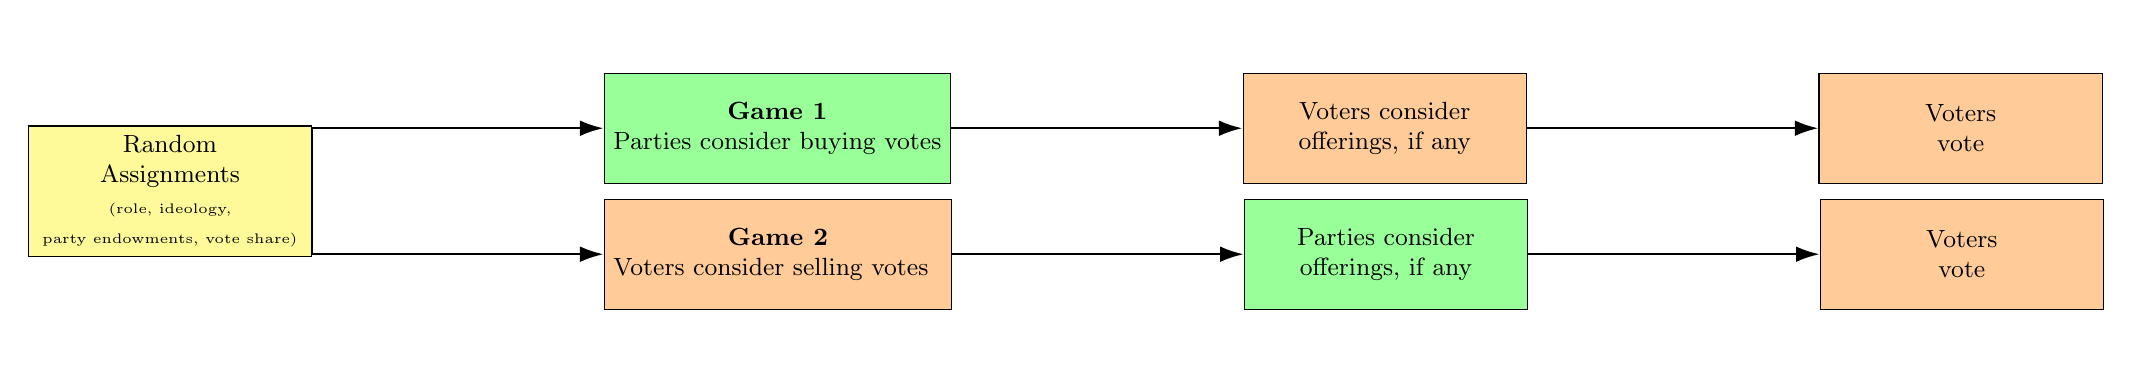
\begin{tikzpicture}[
  node distance=2.8cm,
  every node/.style={font=\small,align=center},
  box/.style={draw,minimum width=3.6cm,minimum height=1.4cm},
  arr/.style={-{Latex[length=3mm,width=2mm]},line width=0.9pt}
]

% ============================================================
% LEFT: Shared Random Assignment Block
% ============================================================

\node[box,fill=yellow!40] (RA) {
    Random\\Assignments\\
    {\tiny(role, ideology,}\\{\tiny party endowments, vote share)}
};

% ============================================================
% GAME 1 PIPELINE (top row)
% ============================================================

\node[above=1cm of RA,font=\bfseries] (G1title){}; %Game 1: Party-initiated vote buying

\node[box,fill=green!40,right=3.7cm of RA,yshift=0.8cm] (G1P) {{\bf Game 1}\\Parties consider buying votes};
\node[box,fill=orange!40,right=3.7cm of G1P] (G1V) {Voters consider\\offerings, if any};
\node[box,fill=orange!40,right=3.7cm of G1V] (G1vote) {Voters\\vote};

\draw[arr] (RA.east) -- ++(0,0.8) |- (G1P.west);
\draw[arr] (G1P.east) -- (G1V.west);
\draw[arr] (G1V.east) -- (G1vote.west);

% ============================================================
% GAME 2 PIPELINE (bottom row)
% ============================================================

\node[below=1cm of RA,font=\bfseries] (G2title){}; % Game 2: Voter-initiated vote selling

\node[box,fill=orange!40,right=3.7cm of RA,yshift=-0.8cm] (G2Vsell) {{\bf Game 2}\\Voters consider selling votes\;\;};
\node[box,fill=green!40,right=3.7cm of G2Vsell] (G2P) {Parties consider\\offerings, if any};
\node[box,fill=orange!40,right=3.7cm of G2P] (G2vote) {Voters\\vote};

\draw[arr] (RA.east) -- ++(0,-0.8) |- (G2Vsell.west);
\draw[arr] (G2Vsell.east) -- (G2P.west);
\draw[arr] (G2P.east) -- (G2vote.west);

\end{tikzpicture}

\end{document}